This test problem is a 1-D problem with two regions with nonzero, uniform
reaction coefficients and sources. The left region has a saturation
value of $\frac{q}{\sigma}=1$, and the right region has a saturation
value of $\frac{q}{\sigma}=0.5$. 
Table \ref{tab:interface} summarizes the test parameters.

%-------------------------------------------------------------------------------
\begin{table}[htb]\caption{Interface Test Problem Summary}
\label{tab:interface}
\centering
\begin{tabular}{l l}\toprule
\emph{Parameter} & \emph{Value}\\\midrule
Domain & $\mathcal{D} = (0,1)$\\
Initial Conditions & $u_0(x)=0$\\
Boundary Conditions & $u(0,t)=u_{inc}=0$\\
Direction & $\mathbf{\Omega} = \mathbf{e}_x$\\
Cross Section & $\sigma(\x)=\left\{\begin{array}{c l}
   \sigma_0, & x\in[x_0,x_1]\\
   \sigma_1, & x\in(x_1,x_2]
   \end{array}\right.,\quad
   \left[\begin{array}{c}\sigma_0\\\sigma_1\end{array}\right] =
      \left[\begin{array}{c}10\\40\end{array}\right]$\\
   & $\left[\begin{array}{c}x_0\\x_1\\x_2\end{array}\right] =
      \left[\begin{array}{c}0\\0.5\\1\end{array}\right]$\\
Source & $q(\x,t)=\left\{\begin{array}{c l}
   q_0, & x\in[x_0,x_1]\\
   q_1, & x\in(x_1,x_2]
   \end{array}\right.,\quad
   \left[\begin{array}{c}q_0\\q_1\end{array}\right] =
      \left[\begin{array}{c}10\\20\end{array}\right]$\\
Speed & $\speed=1$\\
Exact Solution & (Equation \eqref{eq:multiregion_exactsolution})\\
\bottomrule\end{tabular}
\end{table}
%-------------------------------------------------------------------------------

Two studies are performed with this test
problem. The first considers a modification of the analytic solution bounds,
and the second considers upwind solution bounds and the multi-pass limiting
approach described in Section \ref{sec:multipass_limiting}.
Both studies are performed in steady-state with 32 cells.
Table \ref{tab:interface_run_parameters} summarizes the run parameters used
for these studies.

%-------------------------------------------------------------------------------
\begin{table}[ht]\caption{Source-in-Absorber Test Problem Run Parameters}
\label{tab:interface_run_parameters}
\centering
\begin{tabular}{l l}\toprule
\emph{Parameter} & \emph{Value}\\\midrule
Number of Cells & $N_{cell} = 32$\\
Time Discretization & Steady-State\\
Boundary Conditions & Weak with Penalty\\
Penalty Coefficient & $\alpha=1000$\\\midrule
Entropy Function & $\entropy(u) = \frac{1}{2}u^2$\\
Entropy Residual Coefficient & $\entropyresidualcoef = 0.1$\\
Entropy Jump Coefficient & $\entropyjumpcoef = 0.1$\\\midrule
FCT Solution Bounds & Analytic, Modified, Upwind\\
\bottomrule\end{tabular}
\end{table}
%-------------------------------------------------------------------------------

The steady-state analytic solution given by Equation \eqref{eq:analyticDMP}
applied to this test problem are
\begin{subequations}\label{eq:interface_nonupwind_bounds}
  \begin{equation}
      \solutionbound_i^- \le \solutionletter_i
        \le \solutionbound_i^+ \eqc
  \end{equation}
  \begin{equation}
      \solutionbound_i^-
        \equiv 
          \solutionletter_{\min,i} e^{-\dx\reactioncoef_{\max,i}}
            + \frac{\scalarsource_{\min,i}}{\reactioncoef_{\max,i}}
            (1 - e^{-\dx\reactioncoef_{\max,i}}) \eqc
  \end{equation}
  \begin{equation}
      \solutionbound_i^+
        \equiv
          \solutionletter_{\max,i} e^{-\dx\reactioncoef_{\min,i}}
            + \frac{\scalarsource_{\max,i}}{\reactioncoef_{\min,i}}
            (1 - e^{-\dx\reactioncoef_{\min,i}}) \eqp
  \end{equation}
\end{subequations}
The first study considers instead, the tighter solution bounds
\begin{subequations}
  \begin{equation}
      \solutionbound_i^-
        \equiv 
          \solutionletter_{\min,i} e^{-\dx\reactioncoef_{\max,i}}
            + \pr{\frac{\scalarsource}{\reactioncoef}}_{\min,i}
            (1 - e^{-\dx\reactioncoef_{\max,i}}) \eqc
  \end{equation}
  \begin{equation}
      \solutionbound_i^+
        \equiv
          \solutionletter_{\max,i} e^{-\dx\reactioncoef_{\min,i}}
            + \pr{\frac{\scalarsource}{\reactioncoef}}_{\max,i}
            (1 - e^{-\dx\reactioncoef_{\min,i}}) \eqp
  \end{equation}
\end{subequations}
These tighter solution bounds have not been proven analytically; however,
they may still be a decent approximation in practice.
Figure \ref{fig:interface_comparison} shows a comparison of these solution
bounds and the FCT solutions computed using the bounds. For the
original bounds, there are sharp peaks at the interface of the two
regions where the value $\scalarsource_{\min,i}/\reactioncoef_{\max,i}$
becomes overly conservative for the lower bound and similarly for the
upper bound. Results show little or no difference between the FCT
solutions even though the modified bounds lack the peaks at the interface.
In this case at least, it turns out that either there is no antidiffusion
left to go into the interface node, or the solution bounds of neighboring
nodes prohibit any additional antidiffusion into the interface node.
Note that only the reason why the solution bounds differ at nodes other
than the interface node is because of the difference in the iterative
paths taken to obtain the FCT solutions.

%-------------------------------------------------------------------------------
\begin{figure}[ht]
   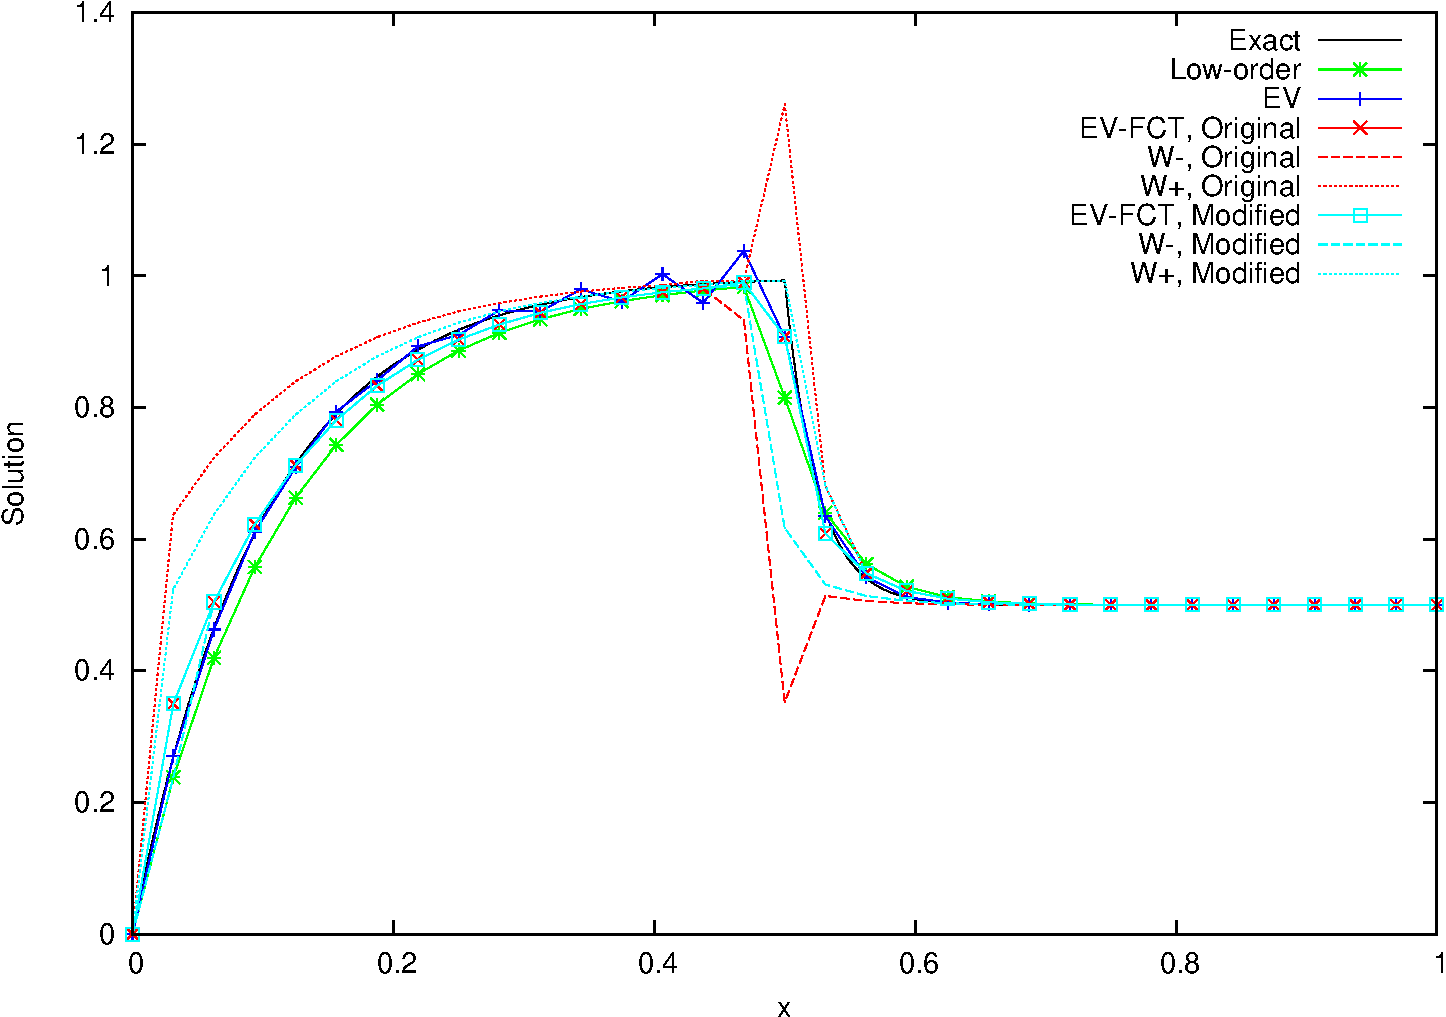
\includegraphics[width=\textwidth]
     {\contentdir/results/transport/interface/images/comparison.pdf}
   \caption{Comparison of Steady-State FCT Solutions for the Interface Test Problem Obtained
     Using Original and Modified Analytic Solution Bounds with 32 Cells}
   \label{fig:interface_comparison}
\end{figure}
%-------------------------------------------------------------------------------

For the second study, the upwind solution bounds given by Equation 
\eqref{eq:local_max_principle} are considered, where here the
node indices are assumed to be ordered left to right:
\begin{subequations}
  \begin{equation}
      \solutionbound_i^-
        \equiv 
          \solutionletter_{i-1} e^{-\dx\reactioncoef_{\max,(i-1,i)}}
            + \frac{\scalarsource_{\min,(i-1,i)}}{\reactioncoef_{\max,(i-1,i)}}
            (1 - e^{-\dx\reactioncoef_{\max,(i-1,i)}}) \eqc
  \end{equation}
  \begin{equation}
      \solutionbound_i^+
        \equiv
          \solutionletter_{i-1} e^{-\dx\reactioncoef_{\min,(i-1,i)}}
            + \frac{\scalarsource_{\max,(i-1,i)}}{\reactioncoef_{\min,(i-1,i)}}
            (1 - e^{-\dx\reactioncoef_{\min,(i-1,i)}}) \eqc
  \end{equation}
  \begin{equation}
    \reactioncoef_{\min,(i-1,i)} \equiv \min\limits_{\x\in(\x_{i-1},\x_i)}
      \reactioncoef(\x) \eqc \quad
    \reactioncoef_{\max,(i-1,i)} \equiv \max\limits_{\x\in(\x_{i-1},\x_i)}
      \reactioncoef(\x) \eqc
  \end{equation}
  \begin{equation}
    \scalarsource_{\min,(i-1,i)} \equiv \min\limits_{\x\in(\x_{i-1},\x_i)}
      \scalarsource(\x) \eqc \quad
    \scalarsource_{\max,(i-1,i)} \equiv \max\limits_{\x\in(\x_{i-1},\x_i)}
      \scalarsource(\x) \eqc
  \end{equation}
\end{subequations}
The second study also considers the multi-pass limitation process described
in Section \ref{sec:multipass_limiting}. Figure \ref{fig:interface_nonupwind}
shows the results for the non-upwind solution bounds given by Equation
\eqref{eq:interface_nonupwind_bounds}, with and without multi-pass limiting,
and Figure \ref{fig:interface_upwind} shows the results for the upwind solution
bounds, with and without multi-pass limiting. The upwind solution bounds
are shown to be much tighter, but the FCT solution with single-pass limiting
is still relatively inaccurate due to the implicit nature of the solution
bounds in steady-state FCT. Multi-pass limiting gives far superior results
in both cases. Note that the multi-pass limiting stopping criteria was that
the total antidiffusion accepted in a pass is less than 1 percent of the
original available antidiffusion. Given that multi-pass limiting produces
superior results, one just needs to consider the additional cost of
this procedure against the benefit. It may be that a more practical multi-pass
limiting procedure can be achieved by using a less strict tolerance.
Table \ref{tab:interface_iterations} gives the number of FCT iterations
required for each considered set of solution bounds for this test problem,
as well as the number of multi-pass limiting passes.
The use of upwind bounds significantly decreases the number of required
iterations; this is because the tighter solution bounds give smaller ranges
for the antidiffusive fluxes. The use of multi-pass limiting appears
to sometimes increase the number of iterations and sometimes decrease
the number of iterations.

%-------------------------------------------------------------------------------
\begin{figure}[ht]
   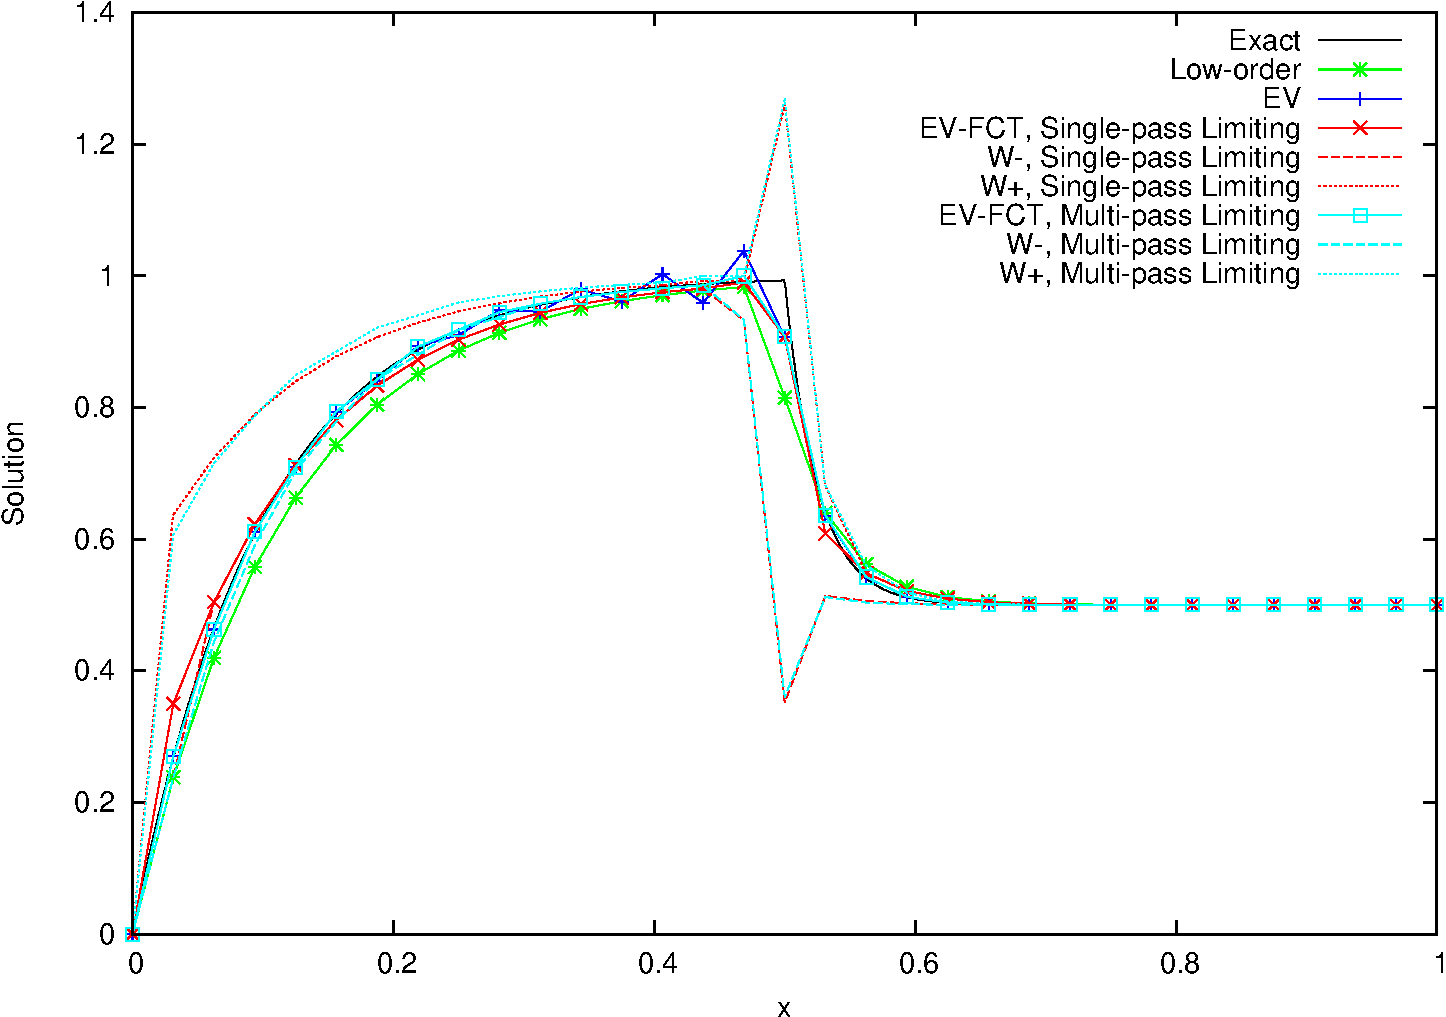
\includegraphics[width=\textwidth]
     {\contentdir/results/transport/interface/images/nonupwind.pdf}
   \caption{Comparison of Steady-State FCT Solutions for the Interface Test Problem
     Obtained with Non-Upwind Analytic Solution Bounds with Single-Pass and Multi-Pass
     Limiting}
   \label{fig:interface_nonupwind}
\end{figure}
%-------------------------------------------------------------------------------
\begin{figure}[ht]
   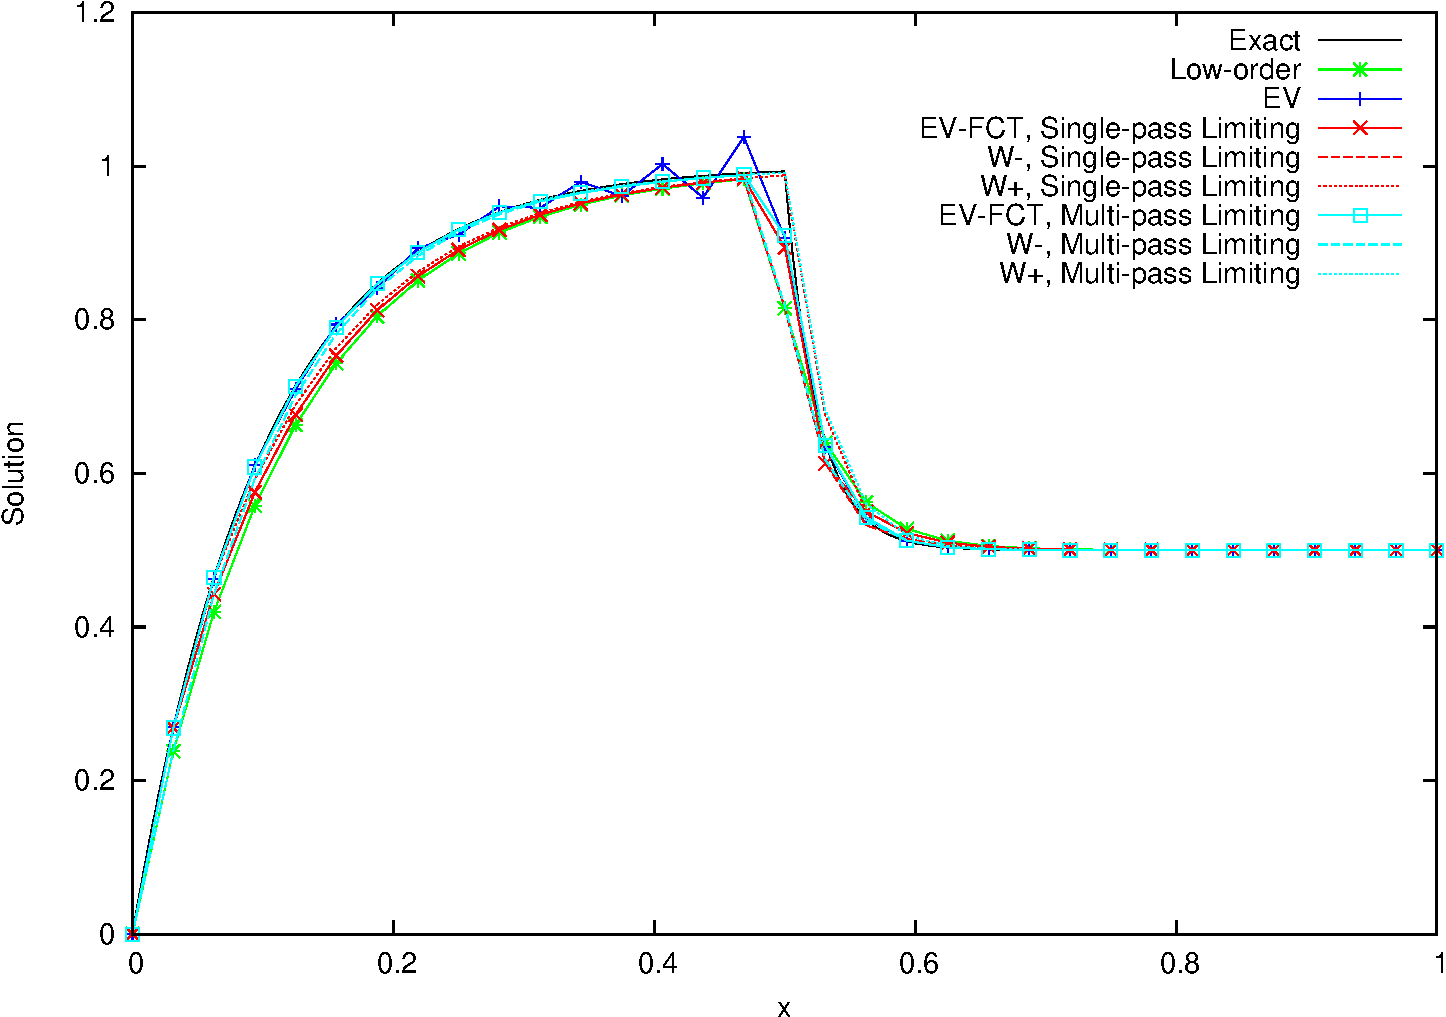
\includegraphics[width=\textwidth]
     {\contentdir/results/transport/interface/images/upwind.pdf}
   \caption{Comparison of Steady-State FCT Solutions for the Interface Test Problem
     Obtained with Upwind Analytic Solution Bounds with Single-Pass and Multi-Pass
     Limiting}
   \label{fig:interface_upwind}
\end{figure}
%-------------------------------------------------------------------------------

%-------------------------------------------------------------------------------
\begin{table}[htb]\caption{FCT Iterations Required for Different Solution Bounds
  for the Interface Test Problem}
\label{tab:interface_iterations}
\centering
\begin{tabular}{c c c}\toprule
\emph{Case} & \emph{Iterations} & \emph{Limiter Passes Per Iteration}\\\midrule
Original Bounds, Single-pass Limiting & 23 & 1\\
Original Bounds, Multi-pass Limiting  & 58 & $\approx 10$\\
Upwind Bounds,   Single-pass Limiting & 15 & 1\\
Upwind Bounds,   Multi-pass Limiting  & 7  & $\approx 19$\\
Modified Bounds, Single-pass Limiting & 23 & 1\\
\bottomrule\end{tabular}
\end{table}
%-------------------------------------------------------------------------------

\clearpage
